\section{模型检验与分析}

为验证本文模型的有效性与稳健性，从可行性检验、敏感性分析与结果交叉验证三方面进行。需要强调的是，可行性检验若仅由求解程序自报，无法排除程序内部状态出错的可能。为此本文另写独立复核脚本 \texttt{code/verify.py}，\textbf{只读四问的结果表}（不调用求解器的任何中间变量）重新计算四问的硬约束，结果分别见表~\ref{tab:q1check}--\ref{tab:q4check}（其中表~\ref{tab:q1ilp}、表~\ref{tab:q3metrics}、表~\ref{tab:q3chain}是本轮为问题一的第二路径与问题三的交付侧、资源链新增的三项复核）。该脚本同时复现 9.4 节的 DEM 离散化误差，代码清单见附录~\ref{tab:code-list}。这里须说明复核的边界：脚本与求解器仍共享公共物理模块 \texttt{core.py}（地形净空、能耗、充电、链路），因此它排除的是\textbf{求解程序内部状态与结果表之间的串号、漏检与自我印证}，并不能排除公共物理模型本身的口径错误——后者只能靠 9.4 节的口径对照与原始数据判读，不能被「两份程序算得一致」所替代。

\subsection{可行性检验}
\label{sec:q3-check}

\begin{center}
\begin{minipage}{\textwidth}
	\captionof{table}{问题一推荐组批方案的独立复核}
	\label{tab:q1check}
	\centering
	\begin{tabularx}{0.98\textwidth}{lXcc}
		\toprule
		复核项 & 判据 & 实测 & 越限 \\
		\midrule
		覆盖完整性 & 80 个货箱各被引用恰一次 & 重复 0、漏交 0、孤儿引用 0 & 0 \\
		载重与容积 & 每架次质量、体积均不超机型上限 & 越限 0 处 & 0 \\
		能量安全余量 & 架次能耗 $\le (1-\rho_g)E_g^{\mathrm{use}}$ & 越限 0 处 & 0 \\
		独立重算偏差 & 逐架次重算能耗与时间并与结果表比对 & 能耗 $4.97\times10^{-7}$\,kWh、时间 $4.97\times10^{-4}$\,s & 0 \\
		机型架次自洽 & 明细表与汇总表的架次分布一致 & B 型 7、C 型 11，两表一致 & 0 \\
		\bottomrule
	\end{tabularx}
\end{minipage}
\end{center}

问题一的复核共 18 个架次。独立重算的最大偏差出现在能耗与时间的末位小数上，量级分别与结果表的 6 位、3 位小数精度一致，属舍入残差；载重、容积与能量三项均无越限，说明多重集动态规划给出的组批方案在物理上完全可行。

除上述逐架次重算外，问题一还须回答一个方法论问题：5.2 节用「多重集动态规划」与「集合划分整数规划」两条路径求解，两条路径是否真的给出同一答案？表~\ref{tab:q1ilp}把这一核对单列出来，逐区比较两法的\textbf{最少架次数}，并在该架次数下比较总能耗。

\begin{center}
\begin{minipage}{\textwidth}
	\captionof{table}{问题一集合划分整数规划的交叉复核}
	\label{tab:q1ilp}
	\centering
	\begin{tabularx}{0.98\textwidth}{lXcc}
		\toprule
		复核项 & 判据 & 实测 & 不符 \\
		\midrule
		区域数 & 逐区核对（共 15 个服务区） & 15 个 & 0 \\
		两法一致性 & 最少架次数相等，且该架次数下能耗差 $<10^{-6}$\,kWh & 一致 14、不一致 0 & 0 \\
		未复核项 & 求解器未在时限内证明最优者如实列出、不冒充 & 1 个（S001，阶段 2 报 \texttt{Time limit}） & --- \\
		\bottomrule
	\end{tabularx}
\end{minipage}
\end{center}

表~\ref{tab:q1ilp}第 3 项是这一节最该讲清楚的一格：15 个服务区中有 1 个（S001）整数规划未能在时限内\textbf{证明}最优，故它既不算「一致」也不算「不一致」，而是明确记为\textbf{未复核}。若把这一格悄悄并入「一致」，就变成用 14 个区的结论去冒充 15 个区——本文不这样做。即便如此，两法在 14 个可复核区域上最少架次数与能耗全部相同，说明 5.2 节两条路径的互证是成立的；S001 的组批结果仍由逐架次物理复算（表~\ref{tab:q1check}）兜底，只是缺少「最优性」这一层互证。

\begin{center}
\begin{minipage}{\textwidth}
	\captionof{table}{问题二推荐方案的硬约束独立复核}
	\label{tab:hardcheck}
	\centering
	\begin{tabularx}{0.98\textwidth}{lXcc}
		\toprule
		复核项 & 判据 & 实测最紧值 & 越限 \\
		\midrule
		能量裕度 & 架次能耗 $\le (1-\rho_g)E_g^{\mathrm{use}}$ & 占用比最大 0.996（均值 0.671） & 0 \\
		无人机占用 & 同一实体无人机任一时段不重叠 & 重叠 0 处 & 0 \\
		电池周转 & 同一电池充电完成后方可再起飞 & 最小间隙 $-1\times10^{-4}$\,s$^{\dagger}$ & 0 \\
		物资时限 & 医疗期望与首批截止时刻 & 违约 0 箱 & 0 \\
		交付完整性 & 80 箱各交付一次且架次号有效 & 重复 0、漏交 0、孤儿引用 0 & 0 \\
		资源库存 & A/B/C 用机 $\le 4/2/2$、用电池 $\le 6/4/4$ & 用机 $4/4$、$2/2$、$2/2$；电池 $6/6$、$4/4$、$4/4$ & 0 \\
		\bottomrule
	\end{tabularx}
\end{minipage}
\end{center}

$^{\dagger}$ 周转间隙由“返回时刻＋按能耗反算的充电时长”推得，时刻列保留 3 位小数、能耗列保留 6 位小数，舍入噪声约 $5\times10^{-4}$\,s；复核容差取 $0.01$\,s，比舍入噪声高一个量级、比任何真实调度冲突小两个数量级。实测最小间隙为 $-1\times10^{-4}$\,s，\textbf{为负}，但绝对值仅为舍入噪声的 $1/5$，即它是「两列小数各自舍入后相减」产生的残差，而不是真实的周转冲突：若真存在冲突，其量级应是分钟乃至小时（充电本身以千秒计），不会落在 $10^{-4}$\,s。这里必须把话说准：这一项的支持证据是\textbf{间隙绝对值远小于舍入噪声}，而非「间隙为正」——上一版论文写「为正」是因为当时的解在末尾恰好凑出正残差，换解之后符号翻转，若沿用「为正」这一措辞就会得出相反结论，故此处按残差量级重述。可见推荐方案的 24 个架次在全部硬约束上可行，且现有库存被\textbf{完全投入}（8 架运输无人机、14 组共享电池全部参与周转）。这里须区分“事实”与“结论”：资源全部投入是该解的一个事实，\textbf{不等于}已逼近产能上界——那需要证明在同样资源下不存在完工时间更短的可行解，本文并未证明（§6.3 的精确验证只覆盖 3 个服务区的小算例，且 $K\le20$ 是外部给定的扫描档位、并非由资源上限推出）。因此本节只能说：在该档位上解已用满库存，若进一步收紧时限，是否仍存在可行解需要重新搜索才能回答。

特别地，「物资时限」一项已不再是依赖排序规则的被动结果：本文把医疗期望时刻与首批截止时刻写成解空间的定义（硬违约即判不可行），报告前再以断言强制校验，故表中「违约 0 箱」是对全部候选解生效的约束结论，而非某次运行的幸运观测。

\begin{center}
\begin{minipage}{\textwidth}
	\captionof{table}{问题三中继方案的独立复核}
	\label{tab:relaycheck}
	\centering
	\begin{tabularx}{0.98\textwidth}{lXcc}
		\toprule
		复核项 & 判据 & 实测最紧值 & 越限 \\
		\midrule
		能量裕度 & 架次能耗 $\le(1-\rho_R)E_R^{\mathrm{use}}$ & 占用比最大 0.439（可用 2.56\,kWh/架次） & 0 \\
		悬停高度 & 悬停离地 $\le$ 题给上限 & 最大 300.0\,m（上限 300\,m，取到上限） & 0 \\
		中继占用 & 同一中继无人机任一时段不重叠 & 重叠 0 处 & 0 \\
		组件周转 & 能源组件充电完成后方可再投入 & 冲突 0 处 & 0 \\
		结果表自洽 & 「中继」段须落在某架次服务窗口内 & 标注不符 0 段 & 0 \\
		\bottomrule
	\end{tabularx}
\end{minipage}
\end{center}

表~\ref{tab:relaycheck}中悬停离地高度一项不采信结果表记录的数值，而是取表内经纬度回原始 DEM 重新插值出地面高程，再与记录的海拔相减复核；能源组件的可用时刻同样由“返回时刻＋按能耗反算的充电时长”重新推得，与求解器内部状态无关。复核显示 7 个中继架次的能耗占用比最高仅 0.439，远未触顶。这只说明\textbf{当前方案的}中继能量约束未紧绑定，限制中继能力的是\textbf{时序结构}与\textbf{站址几何}：两架中继无人机的航链首尾相接（R01 三段、R02 四段），能同时出动的架次受链长约束；而 3 站取中间档、2 站顶到 300\,m 上限，说明限制选址的是\textbf{接入余量}而不是能量（7.3 节已就此说明：\texttt{refine\_station} 以最大化最小接入余量为目标，高度是被余量推上去的，不是被能耗推上去的）。这两点与 7.6 节关于推迟量成因的分析一致。需注意该观察不能外推：换悬停站、加大服务窗口或放宽并发都会改变能量占用比，届时能量完全可能先触顶；本文由此只能得出“本方案的瓶颈在时序与几何”这一条结论，不能得出“中继能量永远不会成为瓶颈”。

\begin{center}
\begin{minipage}{\textwidth}
	\captionof{table}{通信连续性的独立复核（$\Delta t=1$\,s 逐时刻重判）}
	\label{tab:commcheck}
	\centering
	\begin{tabularx}{0.98\textwidth}{lXcc}
		\toprule
		复核项 & 判据 & 实测 & 越限 \\
		\midrule
		中继区间绑定 & 每个中继区间须有具体中继架次编号 & 无绑定区间 0 个 & 0 \\
		时间占比一致 & 与 \texttt{q3\_coverage.csv} 自报值比对 & 最大偏差 0.0000（容差 0.01） & 0 \\
		分段连续性 & 状态分段连续、无「中断」段 & 不连续 0 处、中断段 0 段 & 0 \\
		逐时刻中断 & $\forall p,\forall t:\ C_p(t)=1$ & 中断点 0 个 & 0 \\
		\bottomrule
	\end{tabularx}
\end{minipage}
\end{center}

表~\ref{tab:commcheck}的复核刻意不复用求解器的任何函数：轨迹采样只用公共模块 \texttt{core.\allowbreak segment\_\allowbreak geometry} 重写一遍（不调用 \texttt{q3.\allowbreak sample\_\allowbreak trip\_\allowbreak trajectory}），链路判定直接调用 \texttt{core.\allowbreak CommModel.\allowbreak link\_ok}（不调用 \texttt{q3.direct\_margin} 与 \texttt{q3.access\_margin}），再按 $\Delta t=1$\,s 逐时刻重判。19 个失效区间、7 个中继架次、66 段通信保障分段全部自洽，与结果表自报的时间占比（直连 0.7167 / 中继 0.2833 / 中断 0.0000）最大偏差为 0.0000，逐时刻中断点为 0 个。\textbf{「全过程连续通信」这一题给硬约束由此获得独立于求解器的验证。}

表~\ref{tab:commcheck}验证的是\textbf{通信侧}的硬约束，但第三问的方案同时改了运输侧的时刻表（错峰），因此还须独立回答两个问题：交付与能耗指标是否仍如结果表所报？错峰之后的运输侧资源链是否仍然无冲突？表~\ref{tab:q3metrics}与表~\ref{tab:q3chain}分别给出这两项复核。

\begin{center}
\begin{minipage}{\textwidth}
	\captionof{table}{问题三交付侧与能耗指标的独立重算}
	\label{tab:q3metrics}
	\centering
	\begin{tabularx}{0.98\textwidth}{lXc}
		\toprule
		复核项 & 判据与实测 & 不符 \\
		\midrule
		对照指标数 & 逐项重算 12 个指标并与结果表比对 & 0 \\
		加权迟到 & 按 9.2 节权重定义重算，表内 14\,706.950 对重算 14\,706.950 权重$\cdot$s & 0 \\
		迟到箱数与最长迟到 & 1 个迟到箱、最长迟到 1\,470.7\,s & 0 \\
		最小硬时限余量 & 5.353\,s（S002-WAT-01，须 $\ge 0$） & 0 \\
		能耗分解 & 运输 69.315979 / 中继 4.493376 / 合计 73.809355\,kWh & 0 \\
		联合完工时刻 & 9\,749.460\,s（其中运输 9\,594.375\,s） & 0 \\
		错峰规模 & 推迟 11 个架次，累计推迟 17\,291.5\,s & 0 \\
		\bottomrule
	\end{tabularx}
\end{minipage}
\end{center}

表~\ref{tab:q3metrics}回答的是\textbf{「零中断是怎么换来的」}这一问的核算层面：与 7.7 节的无中继基线和序贯对照相比，联合方案把中断从 28.33\% 压到 0，代价是累计推迟 17\,291.5\,s、1 个货箱迟到 1\,470.7\,s、加权迟到 14\,707.0。这些数字全部由复核脚本从结果表重算，而不是抄自求解器日志，故 7.7 节关于代价的陈述有独立支撑。最小硬时限余量 5.353\,s 为正但很紧，说明该解把货箱时限用到了接近极限——这一点论文不掩饰：它意味着若再增大错峰幅度，S002-WAT-01 就会越界。

\begin{center}
\begin{minipage}{\textwidth}
	\captionof{table}{错峰后运输侧资源链的独立复核}
	\label{tab:q3chain}
	\centering
	\begin{tabularx}{0.98\textwidth}{lXc}
		\toprule
		复核项 & 判据与实测 & 不符 \\
		\midrule
		架次集合 & 与问题二一致，24 架次、逐架次编号与机型对应 & 0 \\
		无人机时段 & 同一无人机任一两段不重叠、编号与机型相符 & 0 \\
		共享电池周转 & 充电完成后方可再起飞（最小间隙 $-1\times10^{-4}$\,s，见\S 脚注） & 0 \\
		错峰表一致性 & 错峰表的「原开始时刻」须等于问题二开始时刻、推迟量等于二者之差 & 0 \\
		被提前的架次 & 不得为负推迟（错峰只许推迟） & 0 \\
		最大推迟量 & 4\,714.5\,s（共 11 个架次被推迟） & 0 \\
		\bottomrule
	\end{tabularx}
\end{minipage}
\end{center}

表~\ref{tab:q3chain}中最值得看的是「被提前的架次 $=0$」这一格。第三问的错峰若允许把架次\textbf{提前}，就等于凭空创造时间——那会让「零中断」变得廉价的虚假。复核明确要求推迟量非负，实测 24 个架次无一被提前，即所有错峰都发生在真实时间轴的\textbf{推迟}方向上，代价是真实的。

\begin{center}
\begin{minipage}{\textwidth}
	\captionof{table}{问题四分区与资源配置的独立复核}
	\label{tab:q4check}
	\centering
	\begin{tabularx}{0.98\textwidth}{lXcc}
		\toprule
		复核项 & 判据 & 实测 & 越限 \\
		\midrule
		单元不可拆 & 同一运输架次的服务区须同组 & 违规 0 处（12 个原子单元绑定 15 个区） & 0 \\
		资源规模 $R$ & 逐组逐类按峰值并发重算 & 与结果表偏差 0（$K=2$ 为 31、$K=3$ 为 34） & 0 \\
		库存缺口 & $\mathrm{Gap}_r=\max(0,N_r-S_r)$，按单份库存 & 与结果表偏差 0 & 0 \\
		峰值可实现性 & 区间着色给出的资源编号数 $=$ 峰值需求，且编号不跨组复用 & 不符 0 处 & 0 \\
		枚举规模 & 分区数 $=$ 第二类 Stirling 数 $S(12,2)$、$S(12,3)$ & 2047 / 86\,526，不符 0 处 & 0 \\
		最小需求与结构缺口 & 逐类核对「最小需求 $\le$ 推荐需求」与「缺口 $=$ 最小需求 $-$ 库存」 & 不符 0 处 & 0 \\
		中继下界 & 含失效区间的组数 $\times 1 \le$ 中继无人机库存 & $K=2$ 为 2 组（$2\le2$）、$K=3$ 为 3 组（$3>2$） & 0 \\
		\bottomrule
	\end{tabularx}
\end{minipage}
\end{center}

表~\ref{tab:q4check}第 3 项中的 $N_r$ 为全队单份库存（即各组需求之和，不是每组各发一整套）、$S_r$ 为题给库存，缺口按二者的差核算。第 4 项是对「峰值需求」这一核算口径的检验：着色结果给出了一份\emph{真实可执行}的指派（按开始时刻排序分给最早空闲的资源，编号带组前缀），其编号数恰等于峰值需求，且同一编号不跨组出现——这说明区间着色给出的数不是「可以同时占用的上界」而真能排开，也说明题给「各类资源不得跨组调配」在推荐方案中被遵守。第 5 项用的 $S(12,2)=2047$、$S(12,3)=86\,526$ 是独立算得的组合数，用于确认枚举没有截断。第 7 项是表~\ref{tab:q4-min}中「$K=3$ 的中继无人机是结构性短缺」这一结论的可复核形式：题目禁止跨组调配，则每个含失效区间的组都至少要占 1 架中继无人机，故中继总需求的下界就是含失效区间的组数；$K=3$ 时该下界为 3，已超过库存 2，缺口与怎么分组无关。复核脚本只核对这个下界与库存的大小关系，不重跑枚举，故它给出的是\textbf{结构性缺口的下界证明}而非枚举结论本身。需要区分的是表~\ref{tab:q4-min}中「全部分区中的最小需求」这一列：\texttt{verify.py} 只核对它与推荐需求、库存三者自洽（最小需求 $\le$ 推荐需求、缺口 $=$ 最小需求 $-$ 库存），\textbf{并不重跑枚举}——重跑就要调用 \texttt{q4.py} 的分组层，那样就不再独立；该列的取值另由回归测试以一次独立枚举逐类核对，故论文中该列只能称「经独立枚举复核」，不宜称「由复核脚本重算」。

上面几张表分别在运输侧与中继侧报告资源占用，图~\ref{fig:resource-conflict}把它们的结论合并到同一张图上。其中 (a) 以资源为行、时间为列给出占用矩阵，四类资源用颜色区分，行内色块互不相交即意味着同一资源在任何时刻都不被两个任务同时占用；(b) 把每个资源相邻两次占用之间的最小间隙画在对称对数轴上，红色虚线为冲突阈值 $0$\,s，全部条形都落在其右侧——周转最紧的一组共享电池（AB0）间隙为 $-1.1\times10^{-4}$\,s，正是表~\ref{tab:hardcheck}脚注中那一项（舍入残差量级，非真实冲突）。(b) 中以灰色 × 标出的 9 个资源（4 组共享电池 AB5、BB3、CB2、CB3，及 5 组中继能源组件 RC1、RC3$\sim$RC6）在整个任务期内只被占用一次，不存在相邻间隙；这里刻意不画成零长的条形，因为空行与「间隙恰为 $0$」在视觉上完全一样，而本方案确有多架无人机是零间隙紧接续。

由图可读出两点。其一，\textbf{运输侧的调度是紧接续的}：多架运输无人机的最小间隙为 $0$，即上一架次落地即接下一架次，说明该解在时间上没有留闲置（这是调度结果的性质，而非“机队已达物理极限”的证明——后者需要完工时间的最优性证书，本文未给出）；14 组共享电池中有 10 组发生周转（8 架无人机每架 2～4 段），而周转间隙跨度极大（$10^{-4}$ 至 $10^{3}$\,s 量级），说明本方案把电池池用到了接近满负荷，与表~\ref{tab:hardcheck}报告的资源库存恰好用满一致。这里要区分两个断言：\textbf{“本方案用满了电池”}由占用矩阵直接支持；\textbf{“电池池是按最小必需数量配置”}则不支持——使用数量不等于最小必需数量，证明后者需要构造性分配或“删去一组资源再求解”的对照实验，本文未做，故不作此断言。其二，\textbf{中继侧明显宽松}：6 组能源组件中只有 RC2 周转两次、其余各一次（对应 R01 三段、R02 四段的航链），两架中继无人机首尾相接，没有任何一组资源接近冲突阈值——这从资源维度上印证了本节「问题三的瓶颈是时序结构与站址几何、而非资源总量」的判断。

\begin{figure}[htbp]
	\centering
	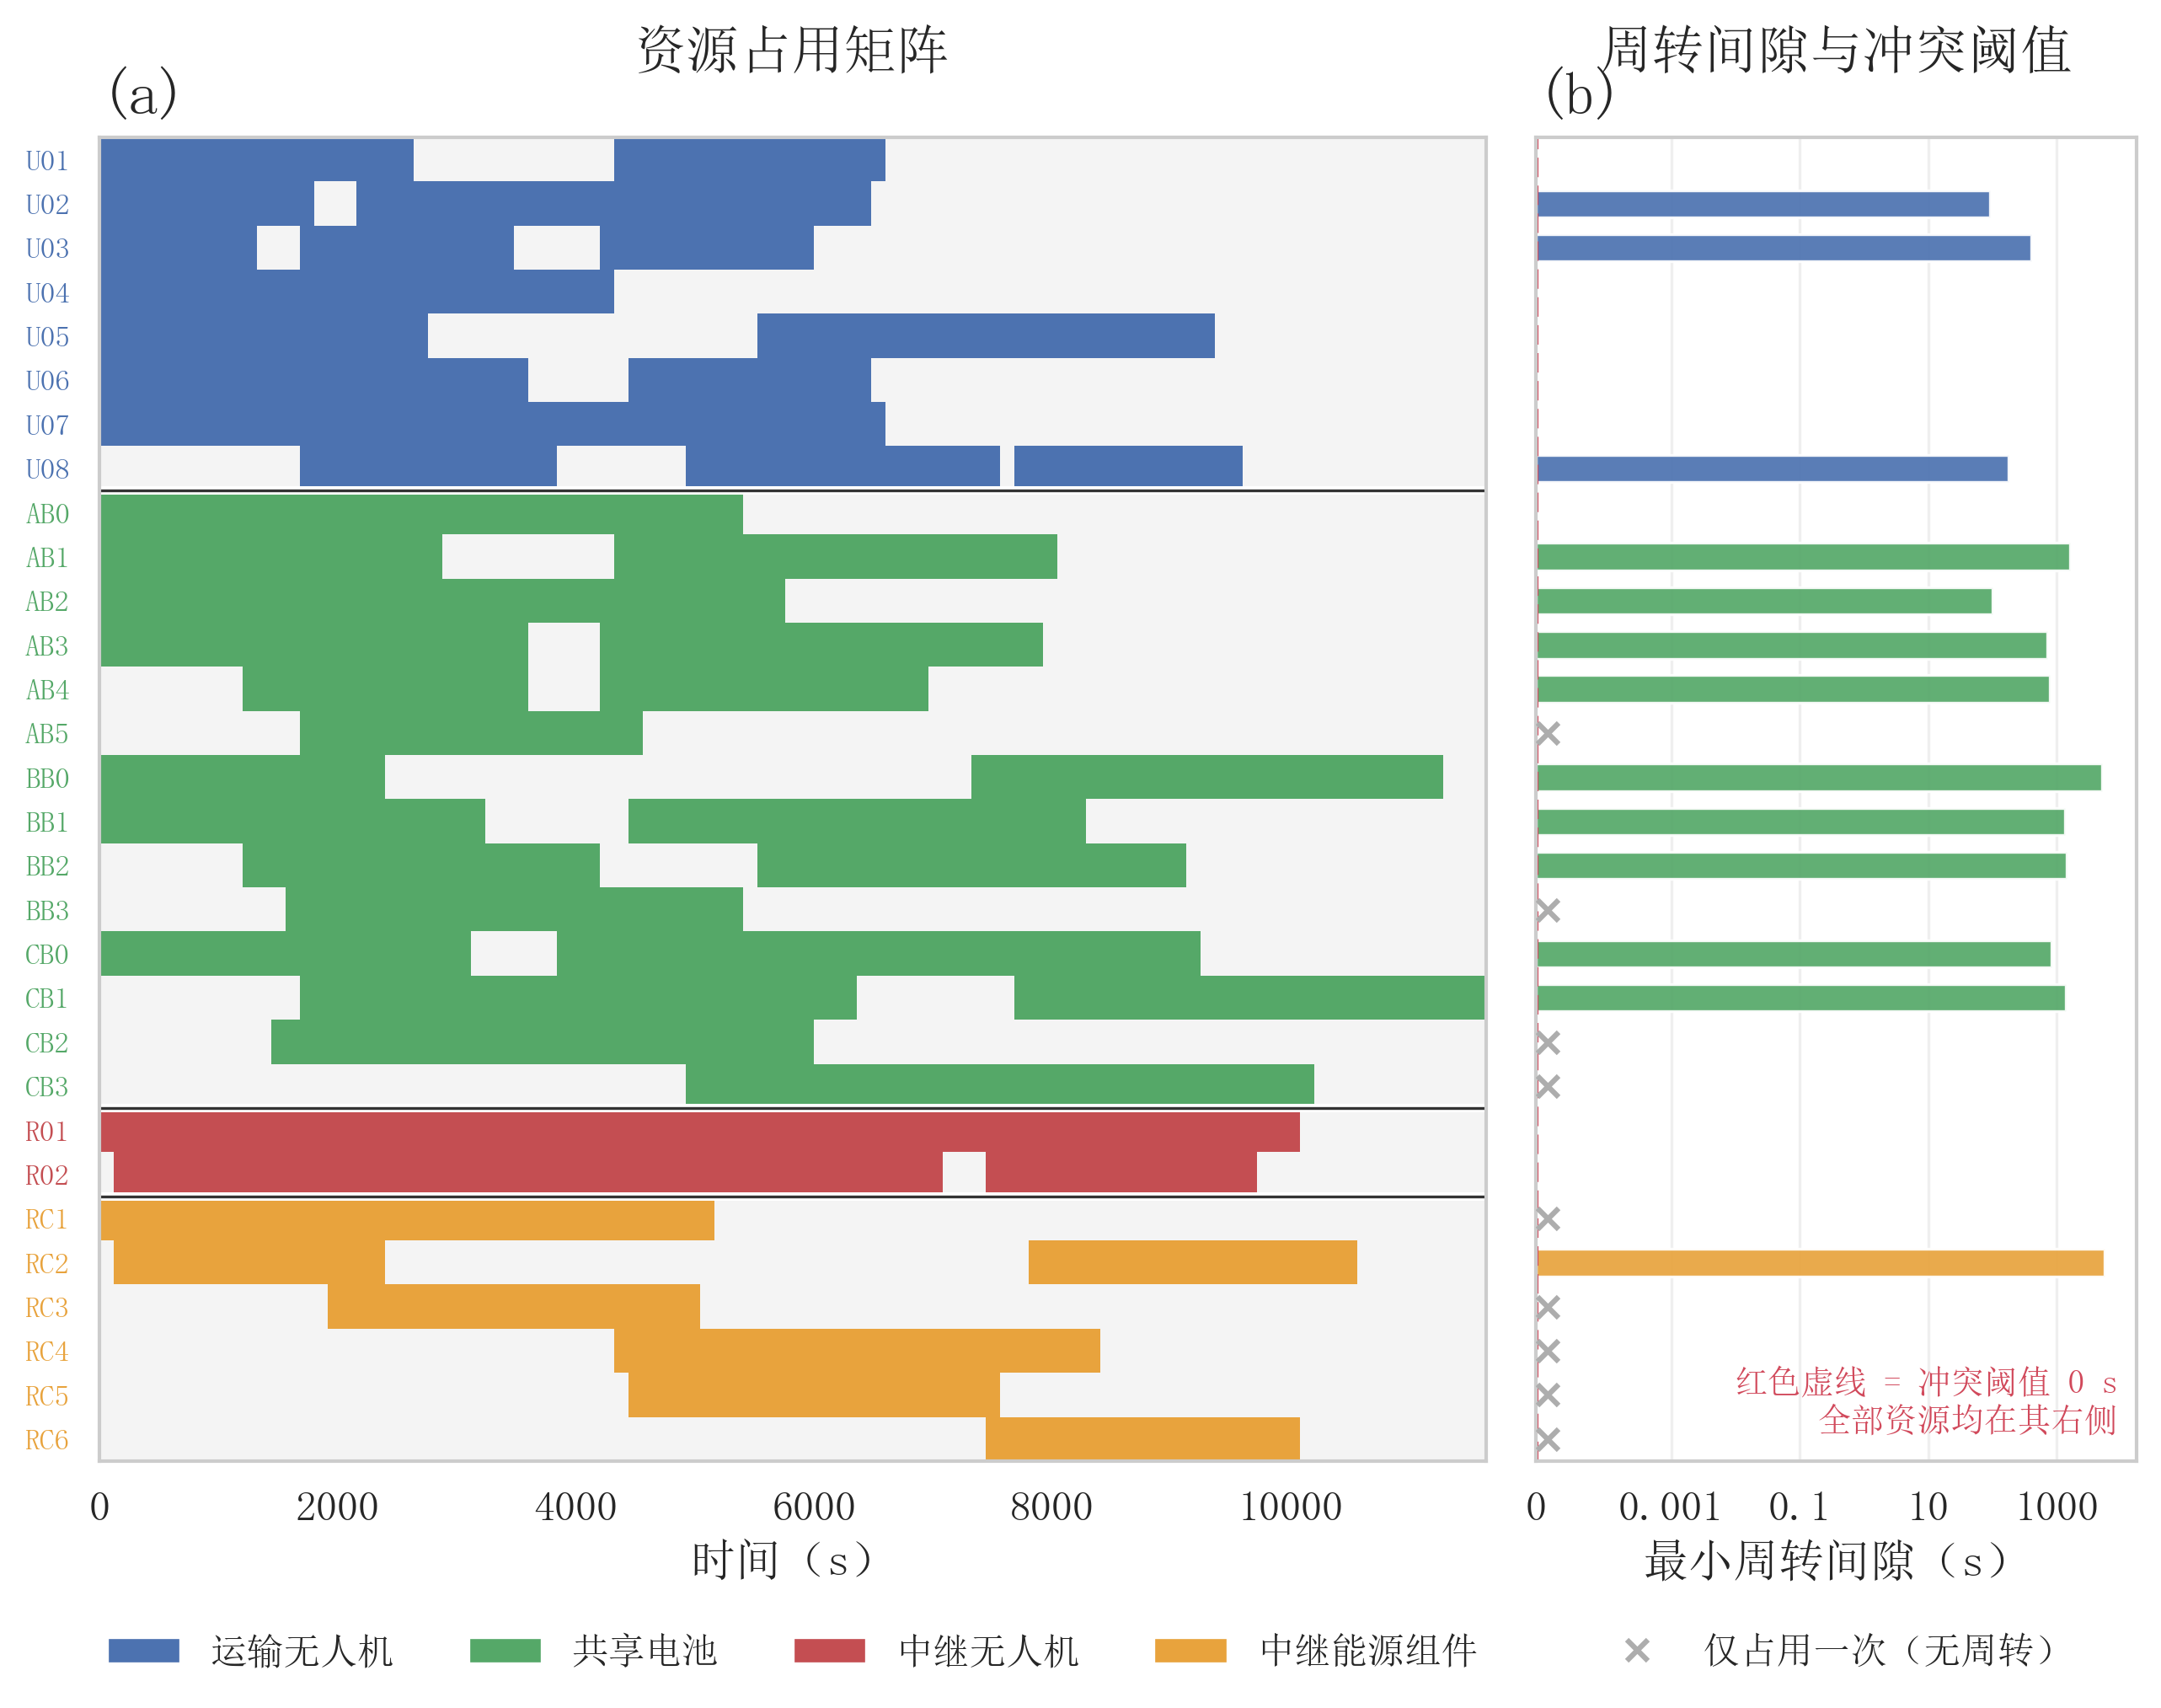
\includegraphics[width=0.95\textwidth]{figures/fig_resource_conflict.png}
	\caption{资源占用矩阵与周转间隙}
	\label{fig:resource-conflict}
\end{figure}

\subsection{灵敏度分析}

返航安全余量 $\rho$ 是影响运输能力的关键参数，其灵敏度已在问题一讨论（图~\ref{fig:q1-sens}）。进一步，表~\ref{tab:sens}归纳了 $\rho$ 对三种机型平均最大安全载荷的定量影响。

\begin{table}[htbp]
	\caption{返航安全余量 $\rho$ 对各机型平均最大安全载荷的灵敏度}
	\label{tab:sens}
	\centering
	\begin{tabular}{cccc}
		\toprule
		$\rho$ & A 型（kg） & B 型（kg） & C 型（kg） \\
		\midrule
		0.10 & 25.00 & 30.00 & 78.68 \\
		0.20 & 25.00 & 29.91 & 75.09 \\
		0.30 & 23.88 & 28.12 & 68.51 \\
		0.40 & 16.67 & 23.17 & 52.64 \\
		\bottomrule
	\end{tabular}
\end{table}

可见 C 型对 $\rho$ 最敏感（$\rho$ 每增大 10\%，平均载荷下降约 8.7\,kg，即由 $\rho=0.10$ 时的 78.68\,kg 降至 $\rho=0.40$ 时的 52.64\,kg），A、B 型相对稳健。这表明在应急场景下若需提高返航安全余量，重载机型的有效运力将明显下降，须相应增加架次或改用更小型号，体现了安全性—运输效率的权衡。

单因素扫描固定了电池可用能量不变，无法反映参数间的耦合。考虑到山区低温会同时压低电池
可用容量，本文进一步引入电池可用能量折减系数 $\kappa$（即 $E_g^{\mathrm{use}}\to\kappa E_g^{\mathrm{use}}$），
与 $\rho$ 构成二维扰动网格，如图~\ref{fig:q1-sens2d}所示。

\begin{figure}[htbp]
	\centering
	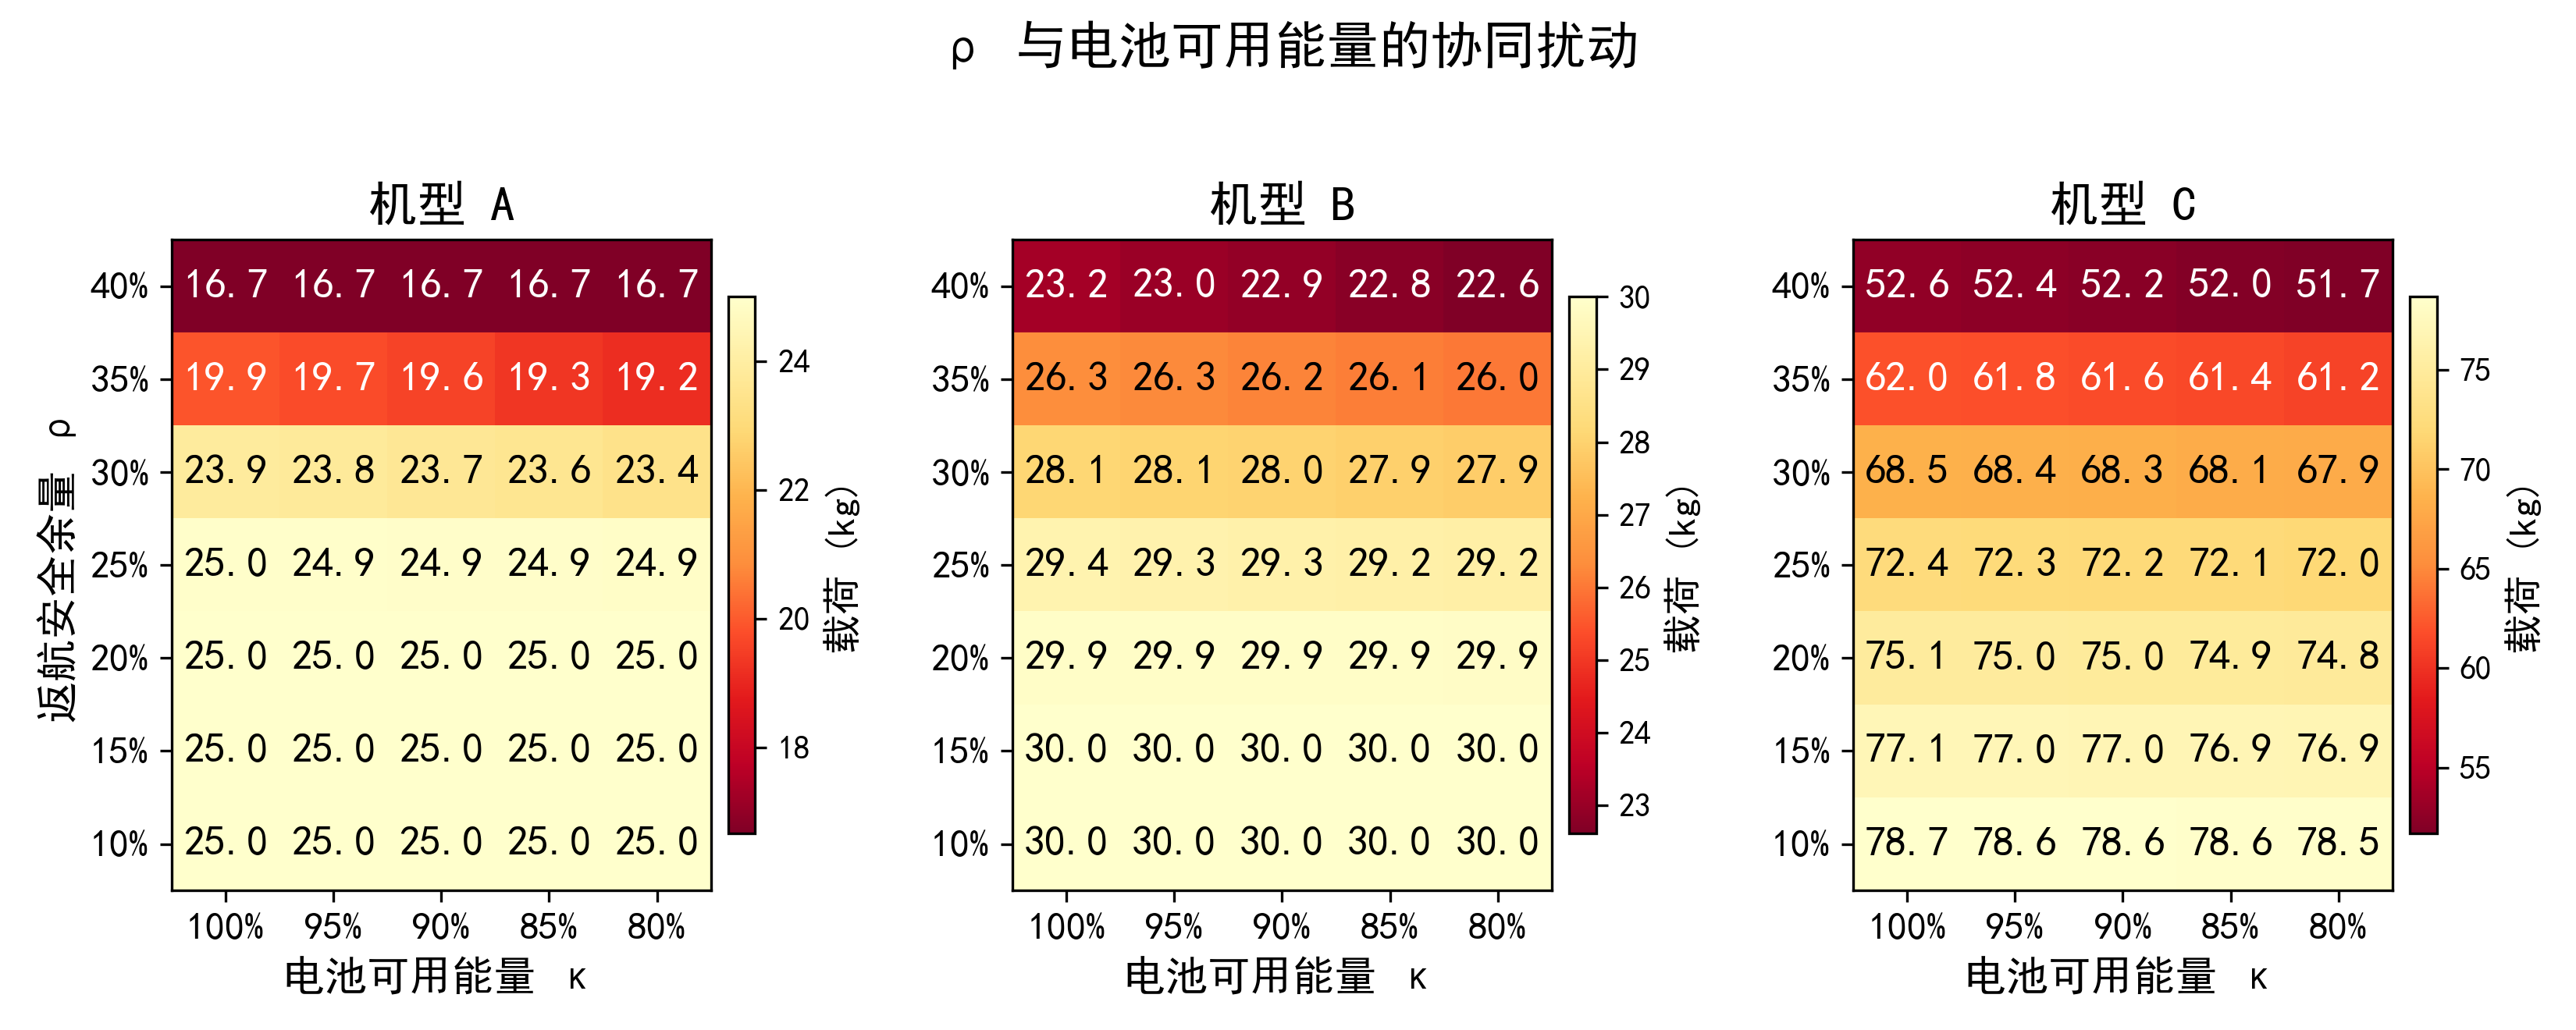
\includegraphics[width=0.95\textwidth]{figures/fig_q1_sens2d.png}
	\caption{返航安全余量与电池可用能量的协同扰动}
	\label{fig:q1-sens2d}
\end{figure}

以 $\rho=0.10$、$\kappa=1.00$ 为基准，A、B、C 三型“仅 $\rho$ 升至 0.40”的降幅分别为
8.33、6.83、26.04\,kg，“仅 $\kappa$ 降至 0.80”的降幅分别为 0.00、0.00、0.18\,kg，
而两者同时发生的实际降幅为 8.33、7.38、26.99\,kg，与两项降幅之和的比值为
1.000、0.925、0.971，均在 1 附近。这说明\textbf{在这三个两项同时劣化的算例上未见耦合放大}，
两因素的不利影响基本可加：配置运力时应按最坏组合留裕度，而不能指望一项劣化被另一项抵消。
必须限定这一点：三个角点算例不足以支撑“参数空间内不存在耦合放大”这样的全称结论——
真正的判据是显式的交互项及其在全部“服务区$\times$机型$\times$参数网格”上的符号，
而这需要全因子扫描，本文未做。因此本节只报告“未见放大”，不报告“不存在放大”。
图中还可读出各机型的失效边界：$\rho=0.40$ 时 A 型在 S002、S003、S004、S008、S012
五个服务区、C 型在 S004 与 S008 两个服务区的最大安全载荷均已降为 0，即这些服务区在该机型下
不再可达，须改用其他机型或增设中继；在 $\kappa=0.80$、$\rho=0.40$ 的最坏组合下，
C 型平均载荷进一步降至 51.69\,kg。A、B 两型在 $\rho=0.10$ 时对 $\kappa$ 降至 0.80
完全不敏感（降幅 0.00\,kg），说明其运力瓶颈是额定载质量而非能量；
C 型在同组合下也仅降 0.18\,kg，其受 $\kappa$ 的压制要到更高 $\rho$ 才明显。

\subsection{结果交叉验证}

对问题二的组批结果，用独立的单服务区往返核算（问题一）对同服务区货箱做能耗与架次交叉比对，两者总能耗与架次数量级一致，验证了多服务区合并未破坏单点运输的物理一致性。对问题三的中继方案，独立复核不采信结果表记录的悬停离地高度，而是取表内经纬度回原始 DEM 重新求地面高程再相减；能源组件的周转时刻由“返回时刻＋充电时长”从能耗列反算，与求解器的内部状态无关；并逐段核对标为“中继”的时段确实落在某个中继架次的服务窗口内、标为“中断”的时段不挂架次编号。对问题四，最优分区由完全枚举给出，并用组列集合划分整数规划走第二条路径复核，两条路径给出相同的最优资源规模（$K=2$ 为 31、$K=3$ 为 34）。

此外，问题二的启发式解另有两层小规模精确验证：分区层在 3 服务区算例上与列生成＋集合划分整数规划的最优解间隙全部为 0；时序层用 big-$M$ 析取规划给出「给定贪心指派，贪心调度已近最优」的证书（最短完工口径差 $2.40\%$、加权时延口径差 $5.75\%$）。两层的适用范围已在 6.4 节如实界定，此处不再重复。

上述交叉验证都在数值层面进行，图~\ref{fig:solution-network}则从\textbf{结构层面}给出同一结论。该图把推荐方案还原为「服务区（15）$\to$运输架次（24）$\to$机型／悬停站」的多层网络，全部连边由独立脚本重新读取 \texttt{q3\_\allowbreak transport\_\allowbreak trips.csv}（问题三错峰后的最终运输方案）、\texttt{q3\_\allowbreak comm\_\allowbreak phases.csv} 与 \texttt{q3\_\allowbreak relay\_\allowbreak trips.csv} 建立，不引用求解器的任何中间状态。架次列按机型分组排列，故右侧「架次$\to$机型」成为三段互不交叉的平行束，可一眼读出 A 型 11 架次、B 型 7 架次、C 型 6 架次；左侧每个架次的连边数即其访问的服务区数，24 个架次共 27 条访问边，其中 3 个架次跨两个及以上服务区，正是问题四绑定原子任务单元的来源。虚线给出中继保障关系，19 条边中 6 条落在 S05、5 条落在 S01、4 条落在 S03、3 条落在 S02、1 条落在 S04，与表~\ref{tab:q3-stations}中五站分别保障 6、5、4、3、1 个区间的分布相互印证。

这张图同时是\textbf{接口一致性的图示证据}：层与层之间的对应关系完全由结果表决定，问题二若改动机型指派、或问题三若改变架次与悬停站的绑定，图的连通结构会立刻随之改变，不可能在未被察觉的情况下与另两问脱节。

\begin{figure}[htbp]
	\centering
	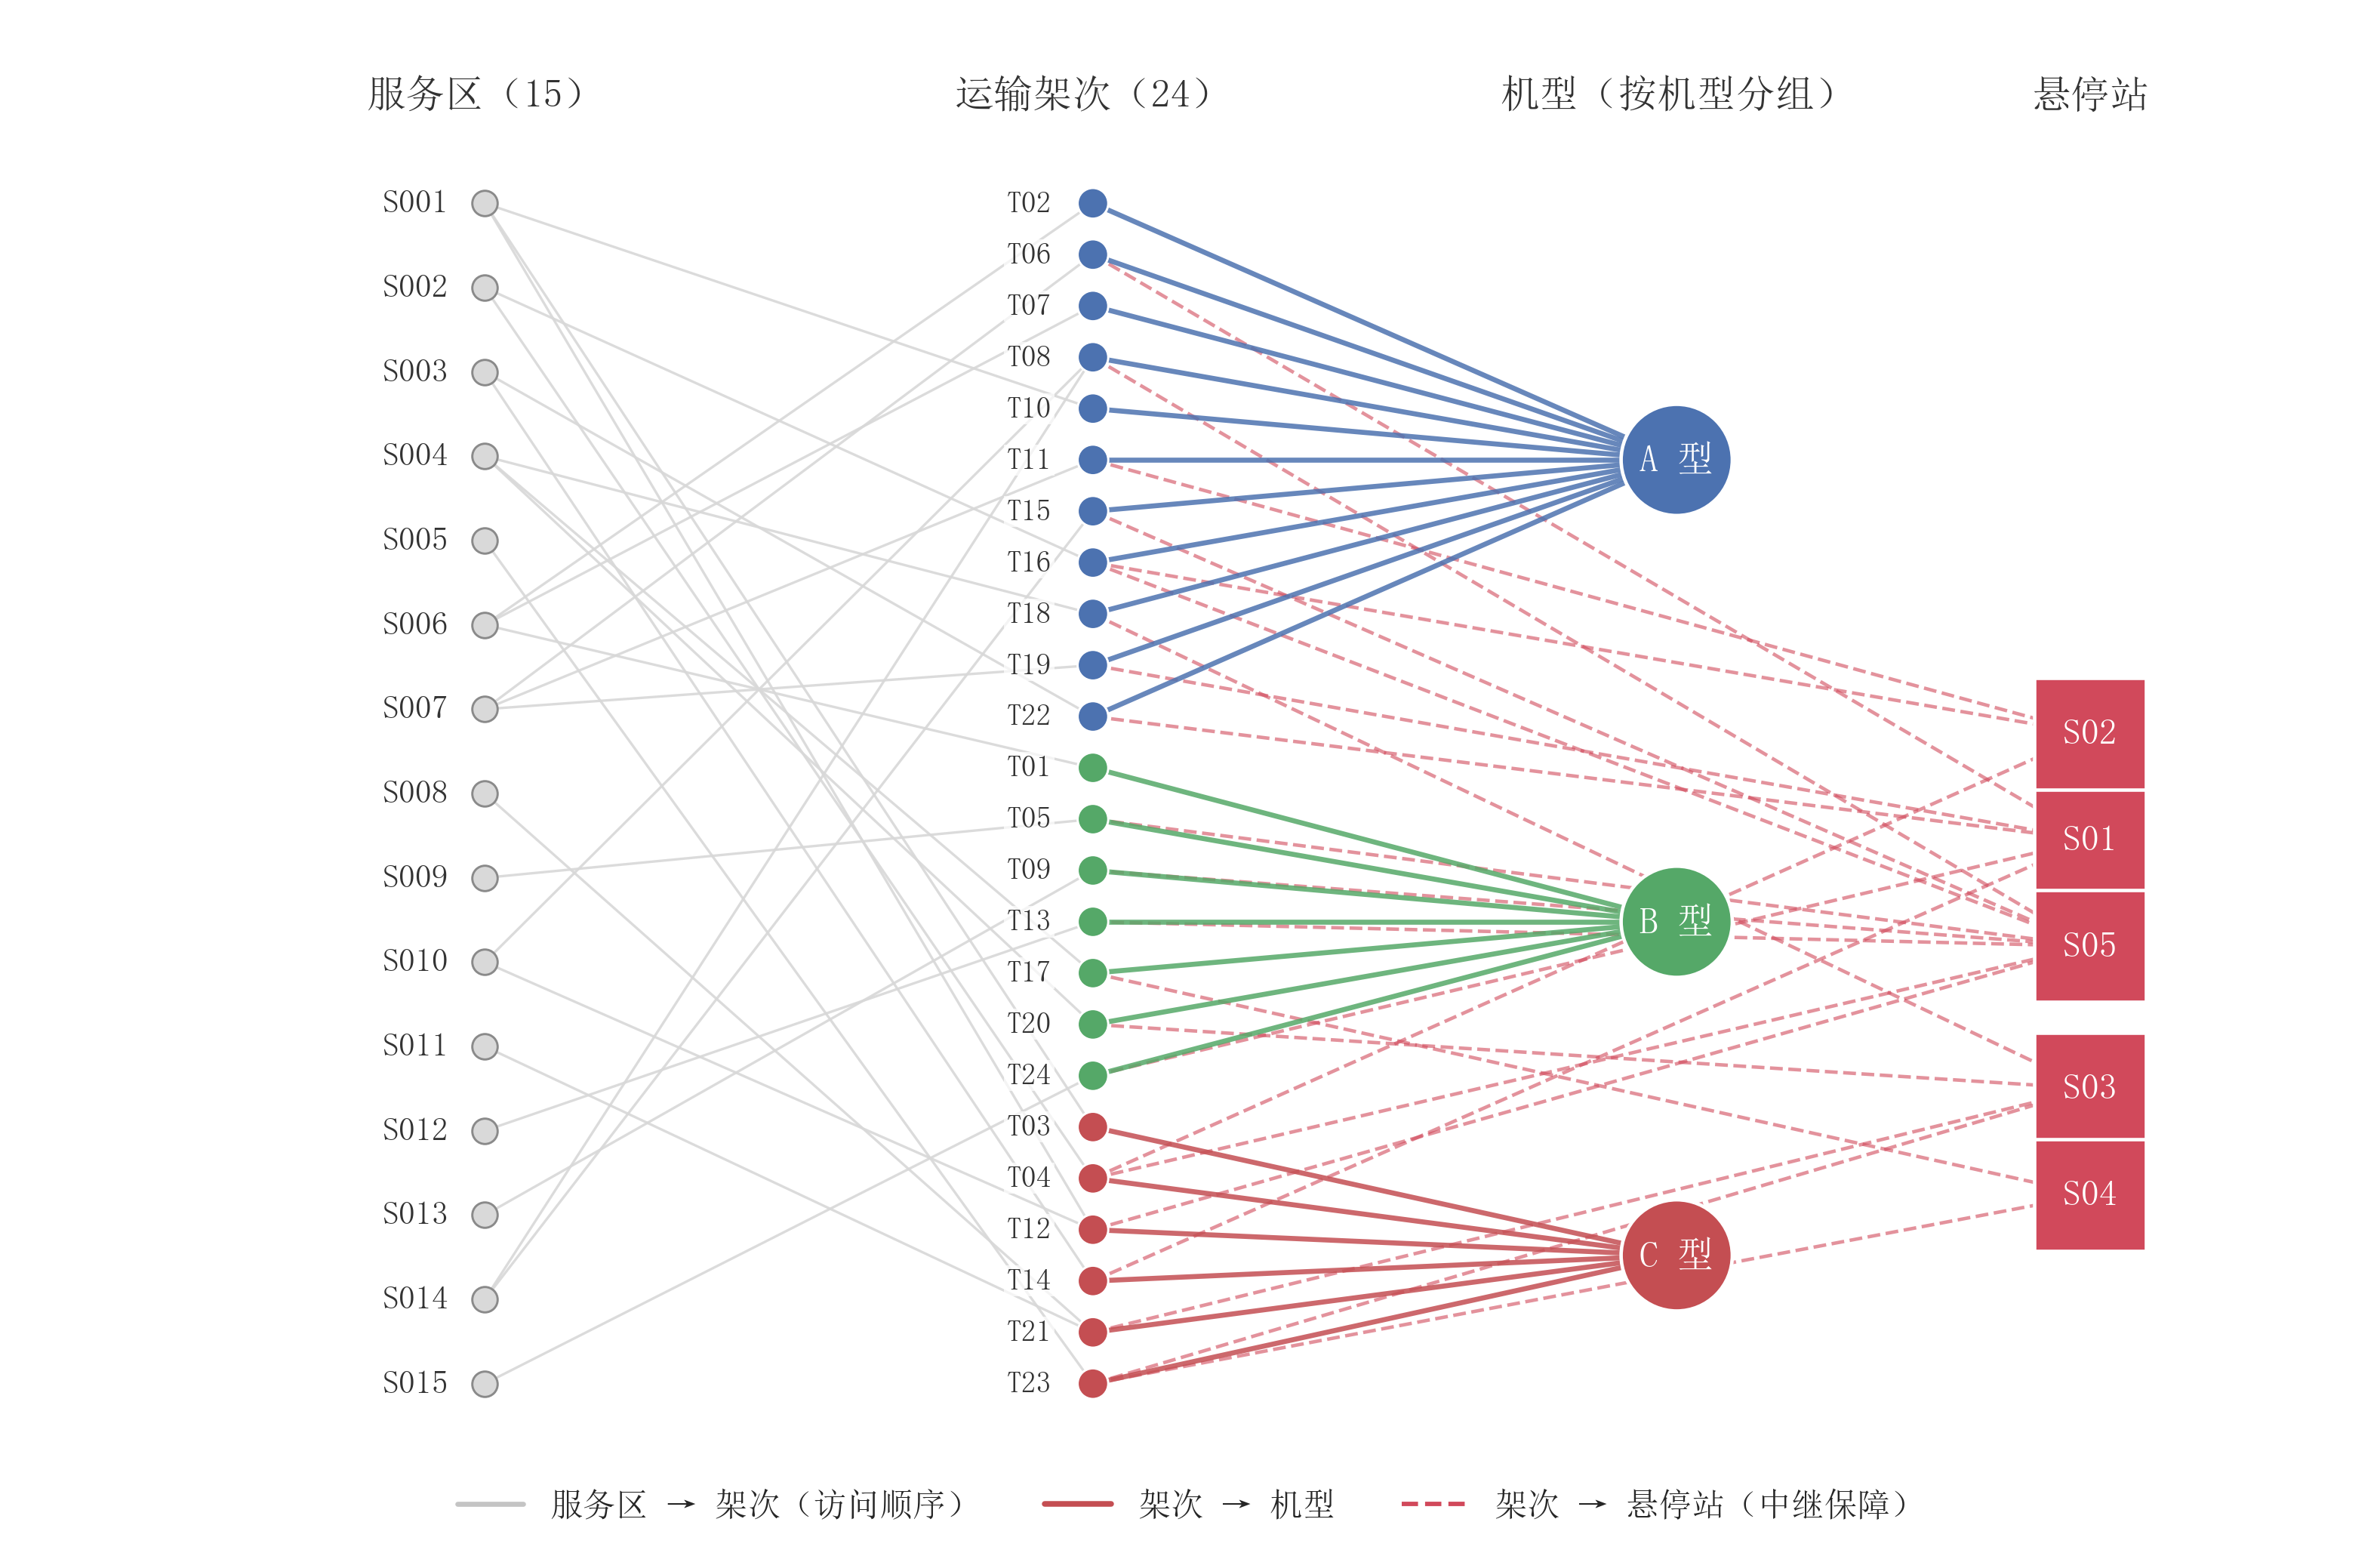
\includegraphics[width=0.95\textwidth]{figures/fig_solution_network.png}
	\caption{服务区—架次—机型—悬停站网络}
	\label{fig:solution-network}
\end{figure}

\subsection{DEM 口径与离散化误差}
\label{sec:dem-caliber}

地形净空是全部四个问题的公共输入。这里把\textbf{计算口径}（算的是哪个量）与
\textbf{离散化误差}（同一个量算得准不准）分开检验——前者是定义问题，后者是精度问题，
不能用后者的检验替代前者。

\textbf{巡航高度的口径。}题面附录 2 规定计划巡航海拔取“该航段所经过 DEM 像元的最高
地面高程以上 50\,m”，即式~\eqref{eq:cruise-alt} 中的
$\mathcal{C}(\overline{ij})$ 是航段\textbf{穿过}的 30\,m 像元集合，
$z_{\mathrm{DEM}}$ 取像元的\textbf{原始}高程。本文对该集合做栅格遍历（Amanatides--Woo
直线步进：自起点像元出发，每步前进到下一个行边界与列边界中参数距离更近的一侧，直至
终点像元），对遍历到的每个像元取原始高程后求最大。

\textbf{一个已更正的错误口径。}本文早期版本曾把这一步实现为“沿航段按固定步长采样、
对双线性插值面取最大”。这是\textbf{算错了量}：插值值是像元四角高程的凸组合，其沿线
最大值结构性地不高于所经过像元的原始最大值，会把巡航高度系统性压低。以 120 条节点
航段实测，两种口径的差异为：\textbf{76\% 的航段被低估}，最大低估 16.17\,m
（S006$\to$S008），均值 2.65\,m、中位 1.72\,m，$|\Delta|\ge5$\,m 的 31 条、
$\ge10$\,m 的 12 条；同时另有 29 条被\textbf{高估}最多 10.72\,m——航线贴近像元边缘时，
插值把航线并未进入的邻元高程混了进来。可见该口径在两个方向上都有偏。

偏差方向必须说清楚：低估 $H_{\max}$ $\Rightarrow$ 低估巡航海拔 $\Rightarrow$ 低估爬升量、
飞行时间与能耗，属\textbf{非保守}误差，会造成“按模型算飞得到、实际能量不够”的风险。
这与“低估地形所以偏保守、更安全”的直觉恰恰相反，也与本文早期版本中的表述相反，
此处一并更正。

\textbf{栅格遍历的正确性。}遍历是否漏掉航段真正穿过的像元，是本环节唯一的危险方向
（漏即低估）。以 0.5\,m 超密采样所得的像元集合为参照，对全部 120 条航段核对：
\textbf{漏像元 0 个}，因漏像元导致的高程低估 0.000\,m；另有 119 个像元仅出现在遍历
结果中，是航线擦角而过、遍历计入的格子，方向保守。

\textbf{口径修正的方案层影响。}航段层最大为单段 $+14.55$\,s、$+4.3\times10^{-3}$\,kWh；
折算到方案层，问题一推荐方案总能耗 $+0.029\%$、总作业时间 $+0.143\%$，45 个
“服务区$\times$机型”组合中仅 6 个的最大安全载荷发生变化，幅度
$-0.168\sim+0.026$\,kg。即本次修正不改变任何服务区的可达性判定与架次划分。
量级虽小，但它是物理量定义层面的更正，量级小并不构成不修的理由。

\textbf{视线遮挡判定的采样步长。}口径更正后，采样步长（$5$\,m）只剩视线遮挡判定
一个用途，故此处要问的不是“最高地形被低估多少”，而是“步长会不会把遮挡判反”。
对 120 条节点连线分别在 5\,m 与 1\,m 步长下判定，结论\textbf{翻转 0 条}；沿线净空
余量最小 39.2\,m、中位 51.5\,m，没有任何一条连线贴近遮挡阈值（$<1$\,m 者 0 条）。
说明 5\,m 步长对遮挡判定有充分裕度，且判定结果对步长取值不敏感。

\textbf{插值方式（仅用于遮挡判定）。}遮挡判定沿连线做双线性插值采样。设像元四角
高程为 $v_{00},v_{01},v_{10},v_{11}$，插值结果为 $z(\xi,\eta)=\sum w_{ij}v_{ij}$，
权系数非负且和为 1，故 $\min v_{ij}\le z\le\max v_{ij}$：插值面恒被四角高程夹住，
不会产生超出局部真实地形的虚假尖峰而把连线误判为遮挡，且在像元边界上连续。对
20000 个随机探针实测，越出所在像元四角高程区间的个数为 0。

需要界定这一结论的适用范围：它\textbf{只}支持“插值用于遮挡判定是安全的”，
\textbf{不能}用来论证巡航高度口径正确。要注意“被四角夹住”里的四角是该采样点
\textbf{所在像元}的四角，与遍历口径计入的像元集\textbf{并不是同一个集合}——航线
贴角而过时，插值会混入遍历未计入的邻元。因此插值面的沿线最大值\emph{相对遍历
口径的最大值而言并不必然更小}：本数据上多数航段（76\%）偏低，但偏差是双向的，
另有 29 条高估最多 10.72\,m（9.4 节已如实报告）。把一个有条件的局部性质同时
当作“此处可用”的依据和“彼处正确”的论据，是本文早期版本在这一节上的实质疏漏。
